\documentclass{article}

\usepackage{graphicx}
\usepackage{listings}
\usepackage{color}
\usepackage[dvipsnames]{xcolor}

\renewcommand\lstlistingname{Quelltext} % Change language of section name

\definecolor{ltgray}{rgb}{0.97,0.97,0.97}

\lstset{ % General setup for the package
    backgroundcolor=\color{ltgray},
    language=C++,
    numberstyle=\tiny,
    frame=tb,
    tabsize=4,
    columns=fixed,
    showstringspaces=false,
    showtabs=false,
    keepspaces,
    captionpos=bf,
    morekeywords={*,
                  cl_int,
                  cl_platform_id,
                  cl_platform_info,
                  size_t,
                  cl_device_type,
                  cl_uint,
                  cl_device_id,
                  scoped_array,
                  cl_context,
                  cl_program 
                },
    commentstyle=\color{blue},
    keywordstyle=\color{magenta}
}

\title{My OPENCL Notes}
\date{2022-12-25}
\author{cgonzalezbrito}

\begin{document}
  \pagenumbering{gobble}
  \maketitle
  \newpage
  \pagenumbering{arabic}
  \section{Introduction}
  
  \iffalse TODO: Put here why i am using two block of code. There are functions that i don't know where they come from. review that \fi

  Usually, the first step is the initialization of OpenCL parameters. The portability approach of the OpenCL standard forces to the programmer to follow a common structure at the beginning of the program. A program in OpenCL must be able to run both in a heterogeneous system that has a device of a vendor (for example a NVDIA GPU), as in another system with a device with similar characteristics but a different vendor (for example a AMD GPU).

  \newpage
  \section{Host Programming}
  
  The program on the host is responsible for the initialization, coordination of kernels execution and data transfer to the kernels. The host creates the initial data buffers that are used by the kernel in charge of normalizing and writing the data into FIFO buffer channels.
  \begin{figure}[h!]
    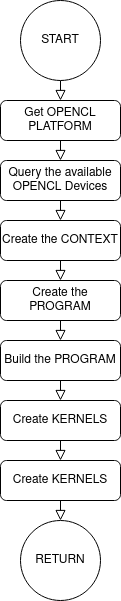
\includegraphics[width=0.2\linewidth]{images/host_diagram.png}
    \centering
    \caption{Host main diagram}
    \label{Fig 1:Host functions main diagram}
  \end{figure}

  \subsection{Get OpenCL Platform}
  Platform is related to the vendor. OpenCL defines a mechanism to identify a specific vendor’s OpenCL implementation in code, i.e. the platform on which the program run. This is important for portability property of OpenCL.
  First, allocate memory for one or more \texttt{cl{\_}platform{\_}id} structures

  \begin{lstlisting}[title={Normal Use}]
  //Allocate memory for one or more cl_platform_id
  //structures.
  cl_int clGetPlatformIDs(
              cl_uint num_entries,
              cl_platform_id *platforms,
              cl_uint *num_platforms
              )

  //Get platform information.
  cl_int clGetPlatformInfo(
              cl_platform_id platform,
              cl_platform_info param_name,
              size_t param_value_size,
              void *param_value,
              size_t *param_value_size_ret
              )
  \end{lstlisting}

  \begin{lstlisting}[title={Intel Altera use}]
  // Get the OpenCL platform.
  cl_platform_id platform = findPlatform("Altera");
  if(platform == NULL) {
    printf("ERROR:
            Unable to find Altera OpenCL platform.\n");
    return false;
    }
  \end{lstlisting}

  \subsection{Query the available Devices}
  Devices are related to the hardware (FPGA, GPU, etc.) that runs kernels code. This works as like the \texttt{clGetPlatformIDs} function. 

  \begin{lstlisting}[title={Normal Use}]
  //Create the devices structures
  cl_int clGetDeviceIDs(cl_platform_id platform,
                        cl_device_type device_type,
                        cl_uint num_entries,
                        cl_device_id *devices,
                        cl_uint *num_devices)

  //Get platform information.
  cl_int clGetPlatformInfo(cl_platform_id platform,
                           cl_platform_info param_name,
                           size_t param_value_size,
                           void *param_value,
                           size_t *param_value_size_ret)
  \end{lstlisting}

  \begin{lstlisting}[title={Intel Altera use}]
  // Query the available OpenCL devices.
  scoped_array<cl_device_id> devices;
  devices.reset(getDevices( platform,
                            CL_DEVICE_TYPE_ALL,
                            &num_devices)
                        );
  device = devices[0];
  \end{lstlisting}

  \subsection{Create the CONTEXT}
  After query the number of the devices available, the context is created. The context is the set of devices which can work together. The context makes possible the command queue structure. The devices in context must be of the same platform.

  \begin{lstlisting}[title={Normal Use}]
  cl_context context = clCreateContext(
              const cl_context_properties *properties,
              cl_uint num_devices,
              const cl_device_id *devices,
              (void CL_CALLBACK *notify_func)(...),
              void *user_data,
              cl_int *error
              )

  // OR 

  cl_context context = clCreateContextFromType(
              const cl_context_properties *properties,
              cl_device_type device_type,
              (void CL_CALLBACK *notify_func)(...),
              void *user_data, cl_int *error
              )
  \end{lstlisting}

  \begin{lstlisting}[title={Intel Altera use}]
  // Create the context.
  cl_context context = clCreateContext(
              NULL, num_devices,
              &device, NULL, NULL, 
              &status
              );
  checkError(status, "Failed to create context");
  \end{lstlisting}

  \subsection{Create the PROGRAM and Build it}
  The binaries in \texttt{.aocx} are read and converted in a \texttt{cl{\_}program}. Then, the program is build, that is, it is compiled and linked from the binary file for the specific device in the program context. Listing V is a OpenCL initialization routine for an Altera platform.

  \begin{lstlisting}[title={Normal Use}]
  // {
  clCreateProgramWithSource(
              cl_context context,
              cl_uint src_num,
              const char **src_strings,
              const size_t *src_sizes,
              cl_int *err_code
              )
  
  // OR

  clCreateProgramWithBinary(
              cl_context context,
              cl_uint num_devices,
              const cl_device_id *devices,
              const size_t *bin_sizes,
              const unsigned char **bins,
              cl_int *bin_status, cl_int *err_code
              )

  // }
  // AND
  
  clBuildProgram(
              cl_program program,
              cl_uint num_devices,
              const cl_device_id *devices,
              const char *options,
              (void CL_CALLBACK *notify_func)(...),
              void *user_data
              )
  \end{lstlisting}

  \begin{lstlisting}[title={Intel Altera use}]
  // Create the program.
  std::string binary_file = getBoardBinaryFile(
                KERNEL_FUNC,
                device
                );
  cl_program program = createProgramFromBinary(
              context,
              binary_file.c_str(),
              devices,
              num_devices
              );
  // Build the program that was just created.
  status = clBuildProgram(
              program,
              0, NULL, "", NULL, NULL
              );
  checkError(status, "Failed to build program");
  \end{lstlisting}
\end{document}
